\documentclass[12pt]{article}
\usepackage{paper-scaleformer}
\usepackage{float}
\usepackage{multicol}
\usepackage{esvect}

\newlength\mylen
\newcommand\NextInput[1]{%
	\settowidth\mylen{\KwIn{}}%
	\setlength\hangindent{\mylen}%
	\hspace*{\mylen}#1\\}

\newcommand\NextData[1]{%
	\settowidth\mylen{\KwData{}}%
	\setlength\hangindent{\mylen}%
	\hspace*{\mylen}#1\\}

%\twocolumn

\begin{document}
\maketitle%

\begin{abstract}
To overcome the quadratic complexity with sequence length of the original transformer, some previous works proposed a kernelized attention mechanism which can scale linearly depending on operation orders. Other works proposed to change the way the position of each token is encoded so that the model depends on relative distance between tokens instead of absolute position. In this work we propose a novel algorithm to combine kernelized attention with relative positional encoding while still scaling linearly in complexity.
\end{abstract}

\clearpage
\begin{multicols}{2}

\section{\label{sec:introduction}Introduction}

\citet{vaswani2017attention} introduced the transformers, a simpler network to model sequence-to-sequence translations tackling new heights of problem complexity. The improvements were due to the non sequential nature of its training process which allowed better parallelization and thus fast training of big models, and due to improved long term dependencies thanks to the intrinsic good gradient flows of the attention mechanism. However the original transformer presented some drawbacks. It has a quadratic complexity with sequences length, what represents a major drawback to its scalability. The positional encoding induce a different initial embedding for the same group of words at different position in the sentence, which is detrimental for generalization. The absolute positional encoding is also detrimental for the extrapolation to sequences longer than training sequences - even for the initially proposed sinusoidal positional encoding.

Ever since, significant research effort have been made to alleviate these problems. Several strategies have been proposed to reduce the quadratic complexity with sequence length, and the relative positional encoding further improved the performances of the model. These improvements have opened the path to the application of transformers to image analysis where scalability and positional invariance are of upmost importance. However most proposed architecture we are aware of only alleviated parts of the issues, by being incompatible with relative positional encoding, having no scheme for masked attention - thus being restrained to encoder-only models, or being complex to use/implement - needing custom operations programmed in CUDA or introducing stochastic methods.

In the present work, by assembling together and building over ideas developed in several works, we propose a complete encoder-decoder transformer model (with unidirectional and bidirectional attention), with linear complexity with regards to sequence length, compatible with relative positional encoding, and that can be implemented with usual functions of neural network frameworks without requiring custom CUDA code.

In the present work we propose a complete encoder-decoder transformer model that scales linearly with large sequence lengths, by putting together ideas developped across several works \cite{vaswani2017attention,shen2020efficient,katharopoulos2020transformers,choromanski2021rethinking,shaw2018selfattention,horn2021translational}. It remains compatible with relative positional encoding, and can be implemented with usual functions of neural network frameworks without requiring custom CUDA code.

\endinput
\begin{figure*}[ht]
	\begin{minipage}{0.48\textwidth}
		\centering
		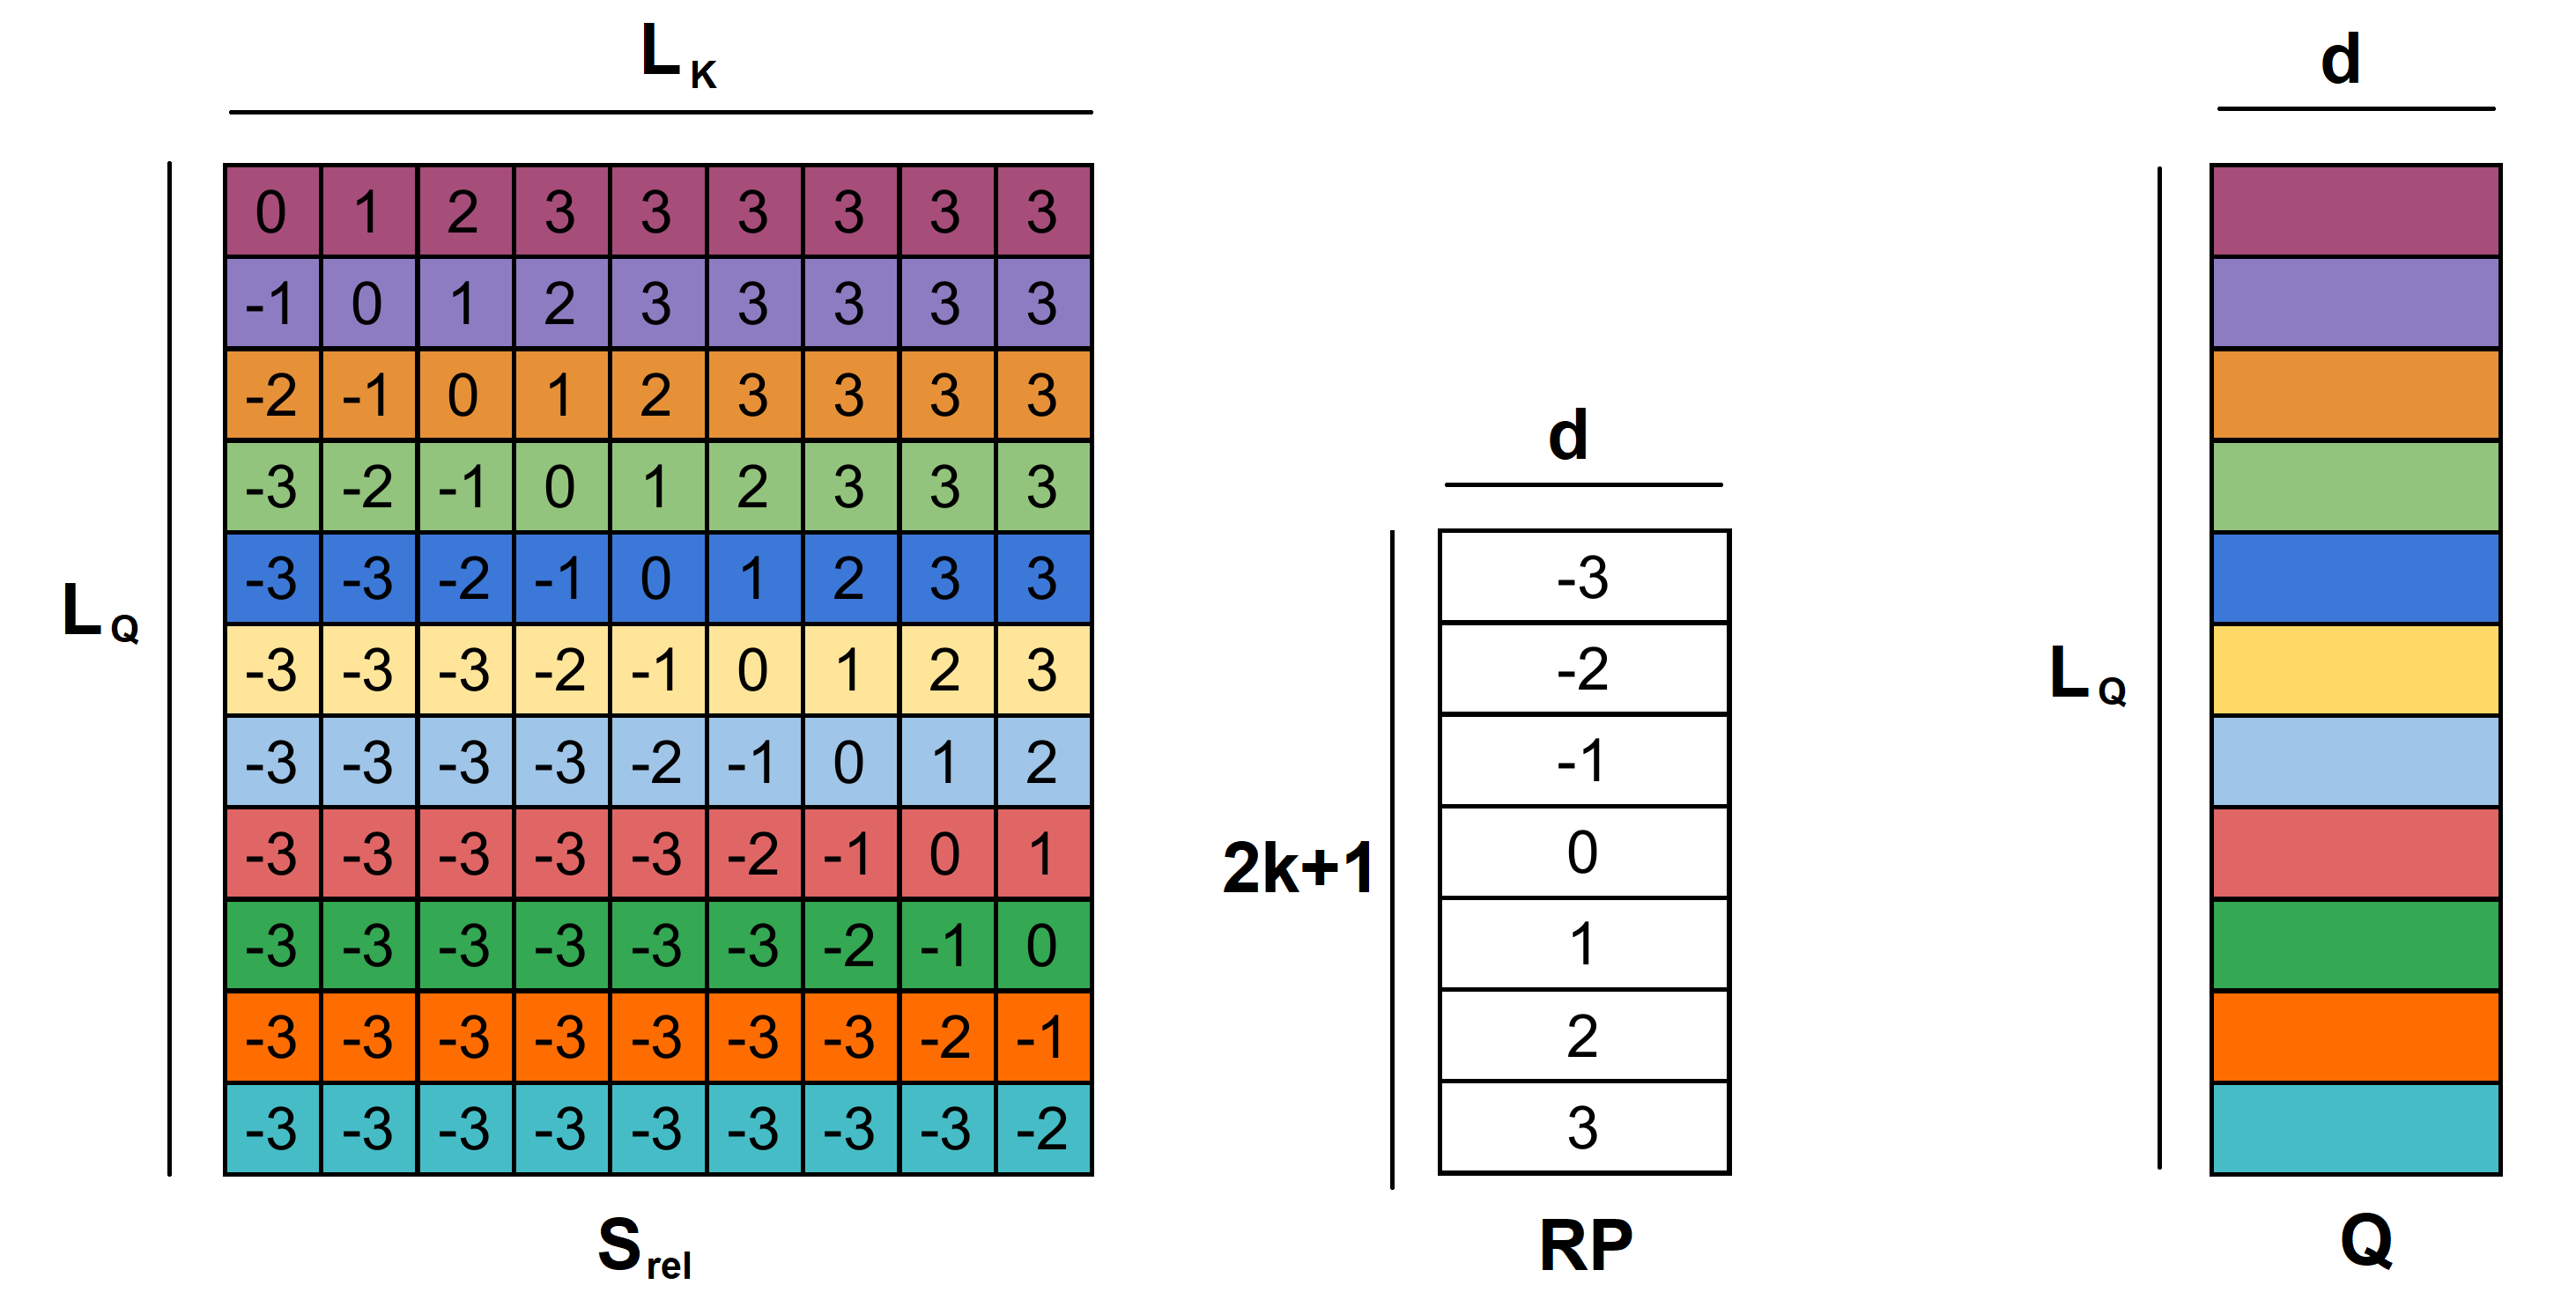
\includegraphics[width=0.9\linewidth]{images/S_rel.png}
		\caption{$S^{rel}$ calculation}
		\label{fig:S_rel}
	\end{minipage}\hfill
	\begin{minipage}{0.48\textwidth}
		\centering
		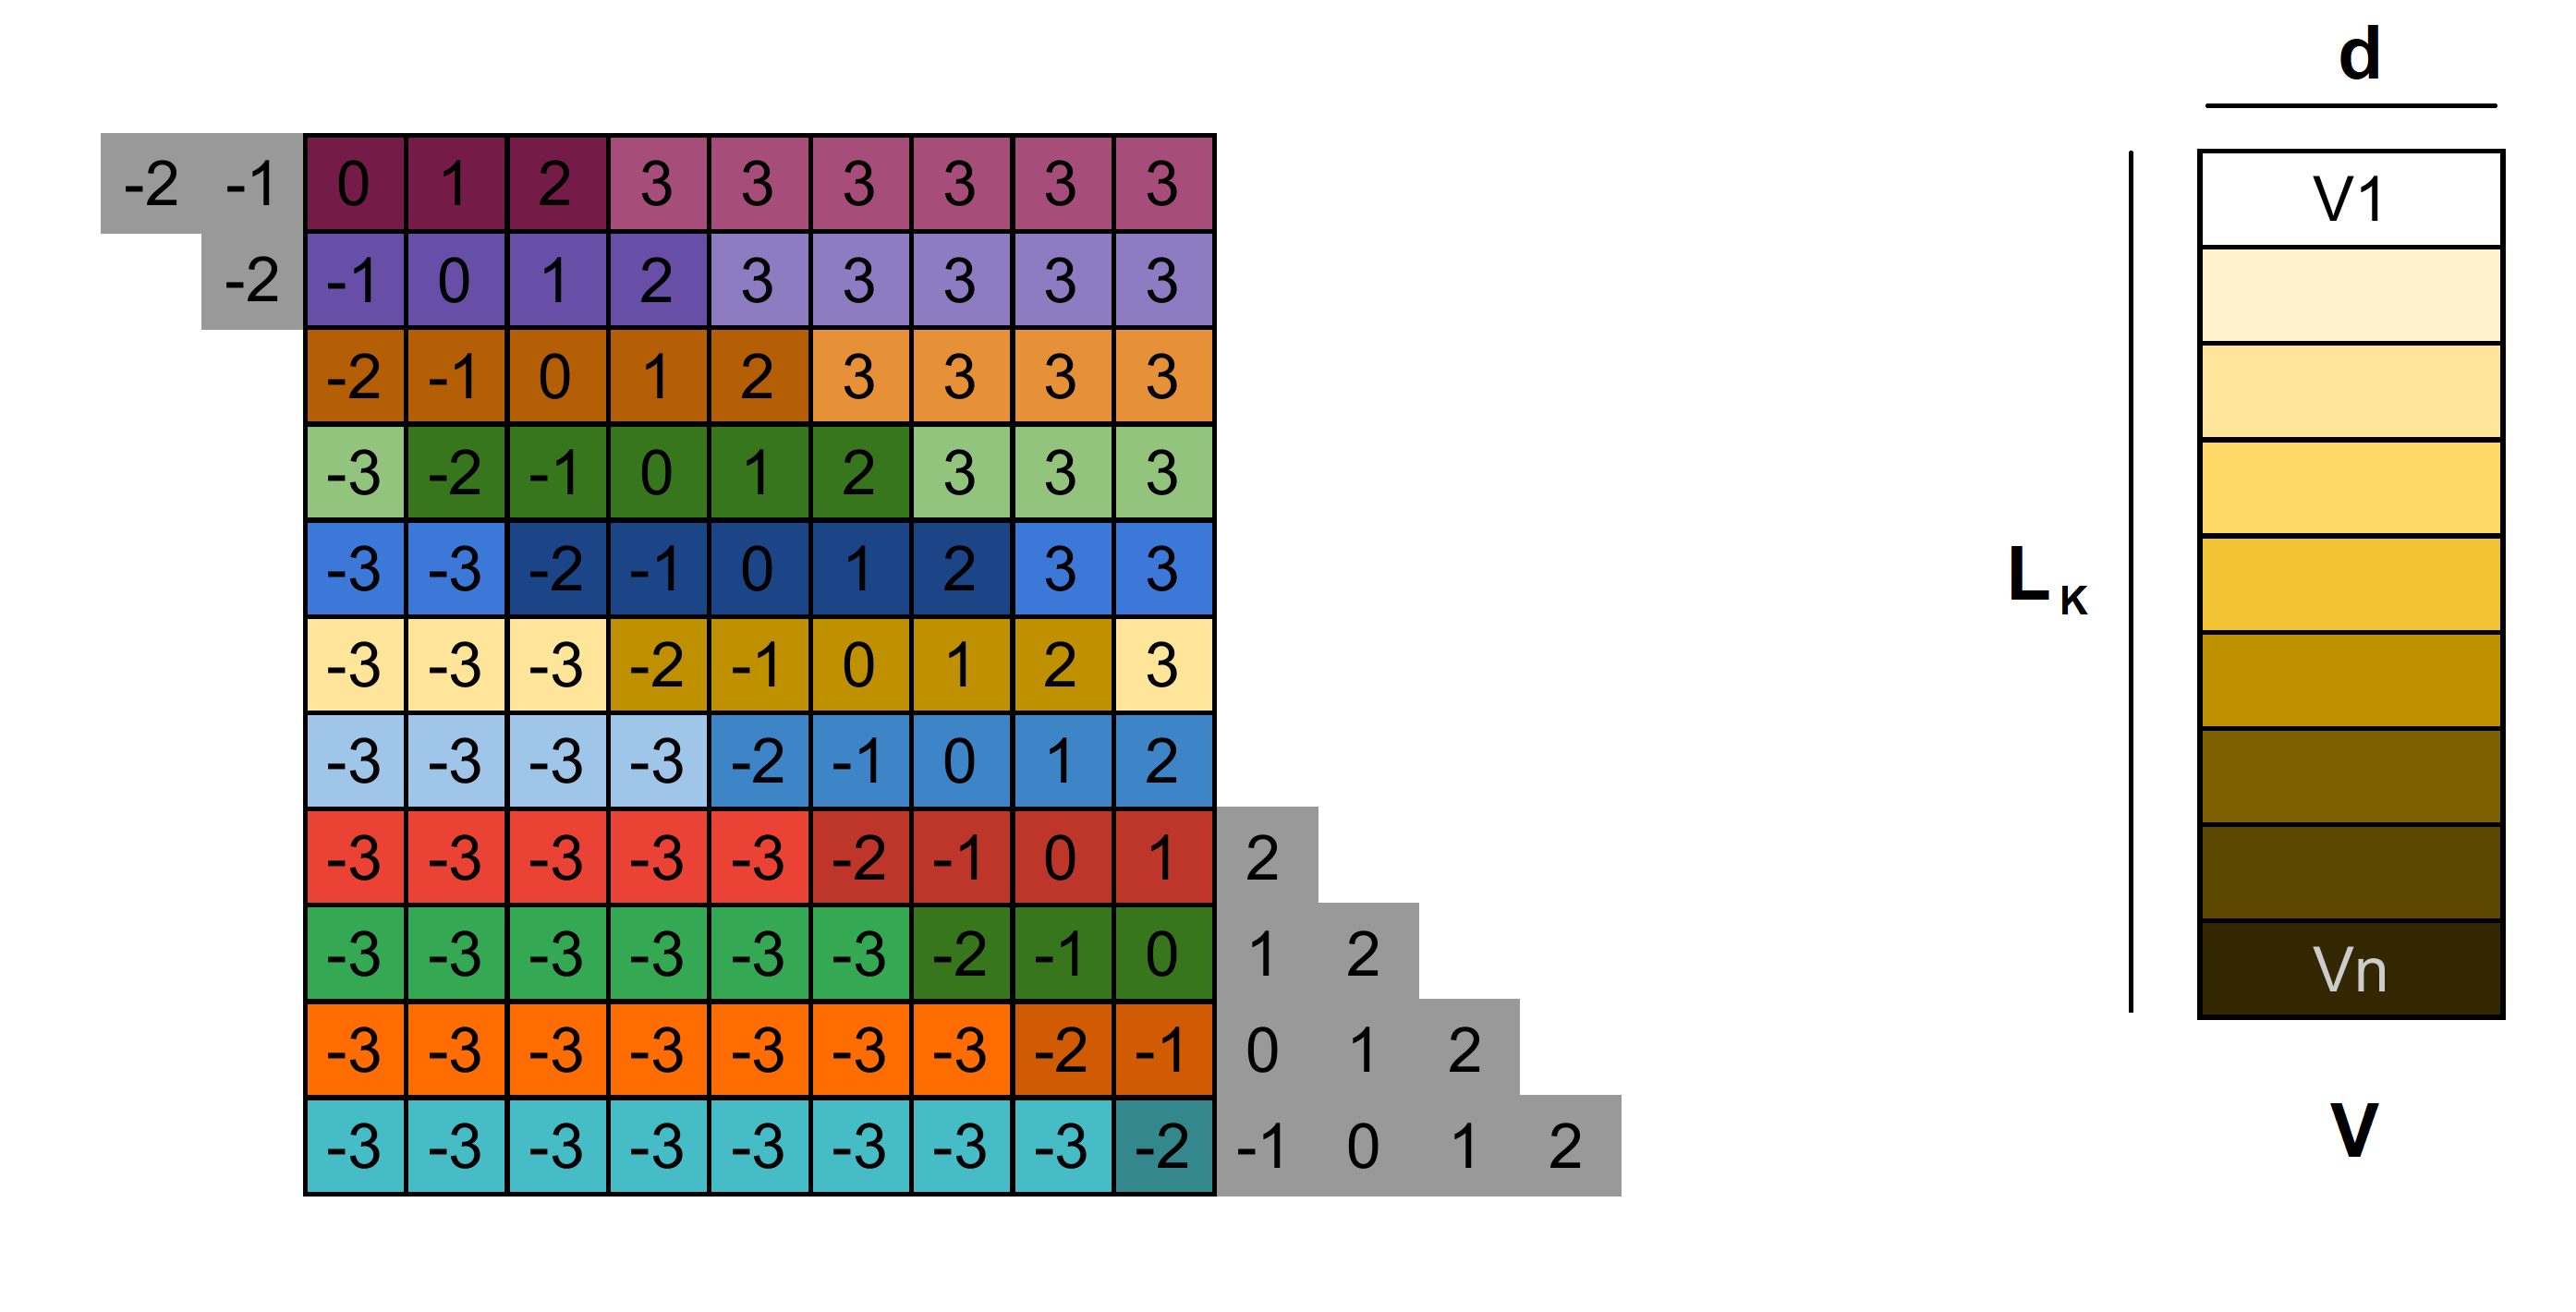
\includegraphics[width=0.9\linewidth]{images/S_rel_V.png}
		\caption{$A^{rel}$ naive calculation}
		\label{fig:A_rel_naive}
	\end{minipage}
\end{figure*}
\section{Background}

\subsection{The original multi-head attention
mechanism}

The scaled dot-product attention proposed by
\citet{vaswani2017attention} transforms the vectorial embedding $\vec{Y}_i$ of a token as a
 function of a sequence of other embedding $\vec{X}_j$. Where
 $\vec{Y}_i$ and $\vec{X}_j$ are all vectors of size $D$. A key
$\vec{K}_j$ and value $\vec{V}_j$ are attributed to each vector
$\vec{X}_j$, and query $\vec{Q}_i$ is attributed to $\vec{Y}_i$.
 The vectors are obtained by linear projection from dimension $D$ to $d$ using three matrices of learnable parameters. The new vector
 $\vec{y}_i'$ is a weighted sum of the $\vec{V}_j$. The weights are
 scores of matching between the query $\vec{Q}_i$ and the keys
$\vec{K}_j$, calculated as the dot product between the two vectors.
They are also \emph{softmaxed} to sum up to 1. The transformation of $L_Q$
vectors $\vec{Y}_i$ as a function of $L_K$ vectors $\vec{X}_j$ can
 be efficiently computed with matrix multiplications:

\begin{equation}
A = \mathrm{softmax}\left(\frac{Q \times K^T}{\sqrt{d}}\right) \times V
\end{equation}

With $Q$ a matrix of shape $(L_Q, d)$, $K$ a matrix of shape
 $(L_K, d)$ and $V$ a matrix of shape $(L_K, d)$. The $\sqrt{d}$
at the denominator is a scaling factor used to avoid saturation in the
exponential terms of the softmax function.

The multi-head attention performs $h$ different projections into spaces
 of dimension $d = D/h$. The resulting vector $\vec{Y}_i'$ is the
concatenation of the $h$ vectors $\vec{y}_i'$ obtained. Thus the
embedding dimension is preserved. Using multiple heads was found
beneficial by the authors over using a single head of dimension
$d = D$.

During training, the cross entropy of the $n^{th}$ predicted token is
 calculated assuming all previous tokens have been generated correctly.
 This enables to parallelize training completely without need for
recurrence. However as the $n^{th}$ token should not depend of the
following tokens, the cells in the upper right corner of the score
matrix are set to $-\infty$ such that after the softmax they are equal
to 0, and the rows still sums up to 1.

\subsection{Improving Transformer scalability with sequence
length}

The original attention mechanism requires the computation of a score
matrix $Q \times K^T$ of shape $(L_Q, L_K)$, with complexity
$O(L_QdL_K)$. If the query and key sequence lengths are multiplied by
two, then the memory used and computation time are multiplied by 4. To
improve the scalability of the transformer with sequence length, several axis of research have been explored.

\citet{kitaev2020reformer} proposed
the Reformer's architecture, which uses an hash-bucketting algorithm to
reduce the complexity of the original multi head attention operation
from $O(L^2)$ to $O(L\log(L))$.

\citet{dai2019transformerxl} proposed the
Transformer-XL's architecture, which cuts the sequence in segments of
length L. The model predicts each stage of the current segment as a
function of the previous and current segment. All the segments are
computed sequentially with a recurrence mechanism. The complexity is linear
with sequence length, but the computation cannot be completely
 parallelized due to the recurrence mechanism, although more than a RNN,
as segments can be computed in one go.

Other publications explored using a sparse attention matrix, such as the
 Longformer by \citet{beltagy2020longformer} and the Big Bird model by
 \citet{zaheer2021big}. As each
token attends to a fixed number of all other tokens, the scalability is
improved. These sparse attention models however require custom
operations implemented in CUDA.

Some other works propose to modify the attention mechanism to be
 compatible with linear complexity. The Linformer by
\citet{wang2020linformer} projects the
 key and values onto a smaller sequence length dimension with matrix
 multiplication. It cannot however generalize to sequences longer than
 during training, as the weights of the projection for such tokens would
 be undefined.

\citet{shen2020efficient} proposed to
 replace the softmax attention score.
 $A = \mathrm{softmax}\left(\frac{Q \times K^T}{\sqrt{d}}\right) \times V$ is
changed into $A = \rho(Q) \times \rho(K)^T \times V$. With $\rho$
the softmax function along the embedding dimension. Thanks to matrix
multiplication commutativity, the order of the operations can be chosen.
If $Q$, $K$ and $V$ are of shape $(L_Q, d)$, $(L_K, d)$ and
$(L_K, d)$ respectively, the complexity of
$(\phi(Q) \times \phi(K)^T) \times V$ is $O(L_Q \times d \times L_K)$ whereas the complexity of
$\phi(Q) \times (\phi(K)^T \times V)$ is
$O\left(max(L_Q, L_k) \times d^2 \right)$. The right-side-first
operation is linear in complexity with sequence length. The shape of the
intermediate result matrix is also changed, allowing to scale the better
in memory requirements as well. The original \emph{softmaxed} attention score
matrix was giving rows of positive scores that sum to 1. With this
change the elements of the score matrix remain positive as $\phi(Q)$
and $\phi(K)^T$ are matrices of positive values, but the rows of the
score matrix does not sum up to 1. This work also does not give a linear complexity formulation for masked attention. If the right-side-first
scheme is adopted, the attention score matrix
$\phi(Q) \times \phi(K)^T$ is never explicitly computed, and can't be
masked.

Building on this idea of commutative attention function proposed by
\citep{shen2020efficient}, \citet{katharopoulos2020transformers} introduced their kernerlized attention function as:

\begin{equation}
A = \frac{\phi(Q) \times \phi(K)^T}{\sum_j \left( \phi(Q) \times \phi(K)^T \right)} \times V
\end{equation}

The function $\phi$ is applied element-wise and can be any positive
function, for example $\phi(x) = elu(x) + 1$. This attention is
row-wise normalized so that all rows of the score matrix are sets of
positive weights adding up to one. This preserves the objective of the
original softmaxed attention scores, while allowing to perform
operations in an optimal order.

The Performer by \citet{choromanski2021rethinking} exploits the same idea of a kernelized attention introduced
by \citet{katharopoulos2020transformers}, with an algorithm that betters approximate softmaxed attention. Most
importantly they also give in annex a prefix sum algorithm to perform
operations in the right-side-first order while giving the same result as
masked left-side-first operation.

Although the author did not specify how to implement it, the only
 implementations we found of this operation requires custom CUDA code. In
 this work we will give an implementation of the right-side-first masked
operation, with usual functions from neural network frameworks, that
remains linear in complexity.

\subsection{Alternatives to absolute positional
encoding}

The original multi-head attention operation introduced by
\citet{vaswani2017attention} was
intrinsically invariant by token order permutation. As token position was
an important information for sequence to sequence models, they encoded
the global position of each token in their embedding. Since then, some
modified attention mechanisms, that depend on relative tokens position,
have been proposed.

\citet{shaw2018selfattention} explored
modifying the attention mechanism so that it depends on the relative
distance between tokens. A second score matrix that is function of the
query and the query/key relative distance is added to the original score
matrix that only depends on query/key vector representation. $A = softmax\left(\frac{Q \times K^T}{\sqrt{d}}\right) \times V$ becomes
$A = \left(\frac{Q \times K^T + S_{rel}}{\sqrt{d}}\right) \times V$ with $S_{rel}$ of shape $(L_Q, L_K)$ defined as
${S_{rel}}_{ij} = \vec{Q_i} \cdotp \vec{RP}_{clip(i-j, -k, k)}$. Where $k$ is the attention horizon length and $\vec{RP}_n$ is one of
$2k+1$ relative positional embedding, vectors of size $d$.
\citet{shaw2018selfattention} and
\citet{huang2018music} observed that introducing this attention scheme improved performances.
The naive calculation of this term however has a complexity of
$O(L_QL_Kd)$. No algorithm was provided to linearize the complexity.

More recently \citet{liutkus2021relative} gives a stochastic positional encoding that is linear in
complexity with regards to sequence length. However the implementation
is complex and its stochastic nature requires that the operations be
repeated several times in parallel.

\citet{horn2021translational} noted that
the term $S^{rel} \times V$ can be computed with linear complexity for
the case where $RP_{-k} = RP_{k}$. However this is restraining as the
model can't make the difference between tokens before the attention
horizon or after.

In this work we will show that the computation of $S^{rel} \times V$
can also be done with linear complexity, without concession.

\endinput

\begin{figure*}[ht]
	\centering
	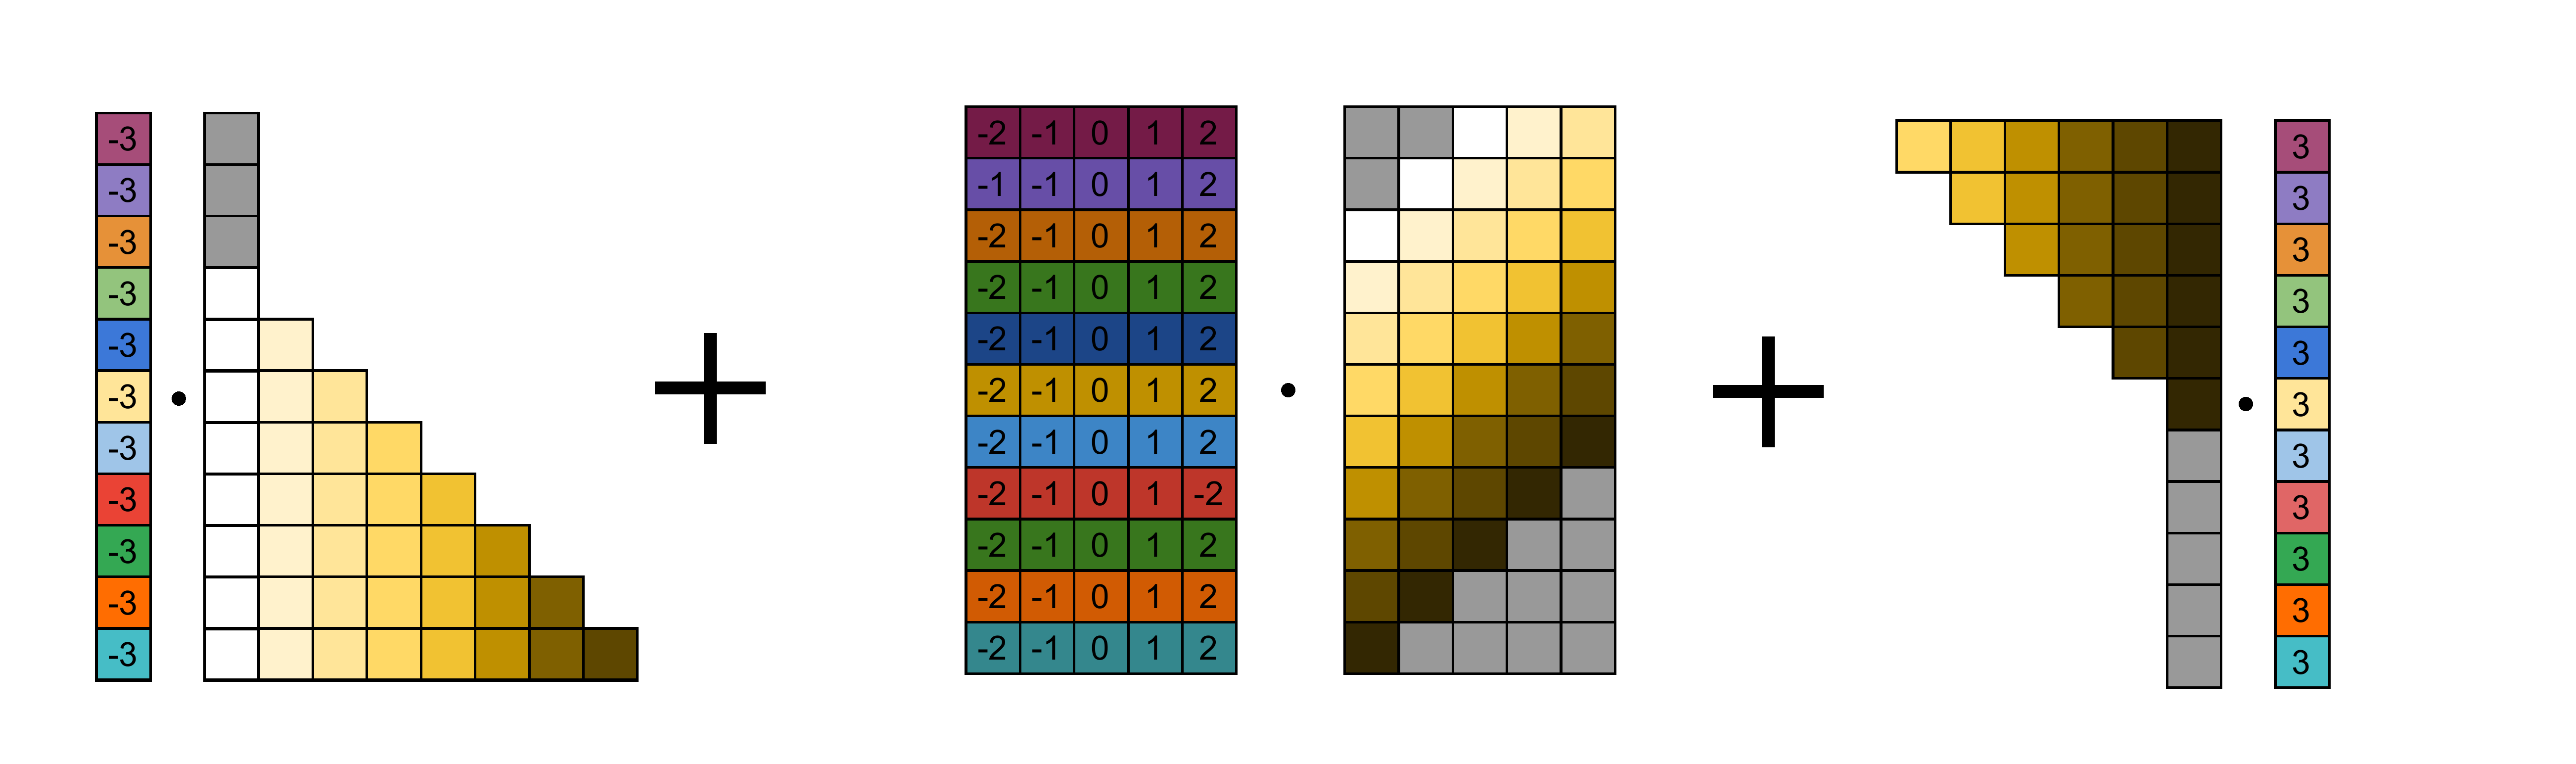
\includegraphics[width=0.9\linewidth]{images/S_rel_V_detailed.png}
	\caption{linear complexity calculation of $A^{rel}$}
	\label{fig:A_rel_linear}
\end{figure*}
\section{Masked attention
implementation}

In this section we will detail the prefix sum algorithm proposed by
\citet{choromanski2021rethinking} for
 masked kernelized attention, and give an implementation with usual
functions of neural network frameworks.

\begin{equation}
A^{masked} = \mathrm{masked} \left( \phi(Q) \times \phi(K^T) \right) \times V
\end{equation}

In this expression, $\mathrm{masked}$ being the operation that set all cells
 above the diagonal to 0 in a matrix. The naive implementation of this
 operation has complexity $O(L_QL_Kd)$.

We can change the complexity using the operation proposed by
 \citet{choromanski2021rethinking}. We
 will derive its formulation here.
 To start with it, $A^{masked}$ is defined as

\begin{equation}
A^{masked} = S^{masked} \times V
\end{equation}

\noindent{}which
in summation form is expressed as

\begin{equation}
A^{masked}_{ij} = \sum_k V_{kj} \times S^{masked}_{ik}
\end{equation}

\noindent{}and the
elements of S are defined as:

\begin{equation}
S^{masked}_{ik} =
\begin{cases}
k \leq i & \sum_l \left( \phi(Q)_{il} \times \phi(K)_{kl} \right) \\
\text{otherwise} &{}0 
\end{cases}
\end{equation}

Putting these elements together leads to

\begin{equation}
A^{masked}_{ij}= \sum_{k=1}^i V_{kj} \times \sum_l \left( \phi(Q)_{il} \times \phi(K)_{kl} \right)
\end{equation}

\noindent{}which can be reworked as

\begin{equation}
A^{masked}_{ij}= \sum_l \phi(Q)_{il} \times \sum_{k=1}^i \left(V_{kj} \times \phi(K)_{kl} \right)
\end{equation}

In this work we make use of these ideas to implement the calculation of
 $A^{masked}$ with complexity $O(max(L_Q, L_K) \times d^2)$ without
 custom GPU code as per the following algorithm:

\begin{enumerate}
\def\labelenumi{\arabic{enumi}.}
\item
$\phi(Q)$, $\phi(K)$, $V$ tensors of shape $(L_Q, 1, d)$,
$(L_K, d)$, $(L_K, d)$
\item
$Unrolled_{kjl} = V_{kj} \times \phi(K)_{kl}$ tensor of shape
$(L_K, d, d)$
\item
$Right = cumsum(Unrolled,\text{ dim=0})$ tensor of shape
$(L_K, d, d)$
\item
$Right = align(Right, L_Q)$ tensor of shape $(L_Q, d, d)$
\item
$A^{masked} = \phi(Q) \otimes Right$ tensor of shape $(L_Q, 1, d)$
\end{enumerate}

\noindent{}with

\begin{itemize}
\item
$\otimes$ the batch matrix product along the last two dimensions
\item
$cumsum(\_, dim=0)$ the function that calculates the cumulated sum
along the first dimension
\item
$align(\_, L_Q)$ the function that extend the first dimensions to
size $L_Q$ by repeating the last element if $L_Q > L_K$, or
truncate to size $L_Q$ if $L_Q < L_K$. (Can be implemented with
slicing and concatenation)
\end{itemize}

\endinput

\begin{algorithm*}[ht]
	\caption{calculation of $A^{masked}$ with linear complexity}
	\label{alg:A_masked}
	\KwIn{$\phi(Q)$ query vectors, tensor of shape $(L_Q, d)$}
	\NextInput{$\phi(K)$ key vectors, tensor of shape $(L_K, d)$}
	\NextInput{$V$ value vectors, tensor of shape $(L_K, d)$}
	\vskip12pt
	\KwData{Expanded tensor of shape $(L_K, d, d)$}
	\NextData{Summed tensor of shape $(L_K, d, d)$}
	\NextData{Aligned tensor of shape $(L_Q, d, d)$}
	\vskip12pt
	\KwResult{$A^{masked}$ tensor of shape $(L_Q, d)$}
	\vskip12pt
	$\text{Expanded}_{kjl} := V_{kj} \times \phi(K)_{kl}$\\
	$\text{Summed} := cumsum\left(\text{Expanded}, \text{dim=0}\right)$\\
	$\text{Aligned} := align(\text{Right}, L_Q, \text{dim=0})$\\
	$A^{masked}_{ij} := \sum_k \left( \phi(Q)_{ik} \times \text{Aligned}_{ikj} \right)$
\end{algorithm*}
\section{Linear complexity RPE
implementation}

In this section we will detail how the relative positional encoding
 proposed by \citet{shaw2018selfattention}
can in fact be computed with linear complexity. The $S_{rel}$ matrix of scores is computed as
${S_{rel}}_{ij} = \vec{Q_i} \cdotp \vec{RP}_{clip(i-j, -k, k)}$. Here
below the colors represent the index of the query and the number the
index of the relative position.

\begin{figure}
\centering
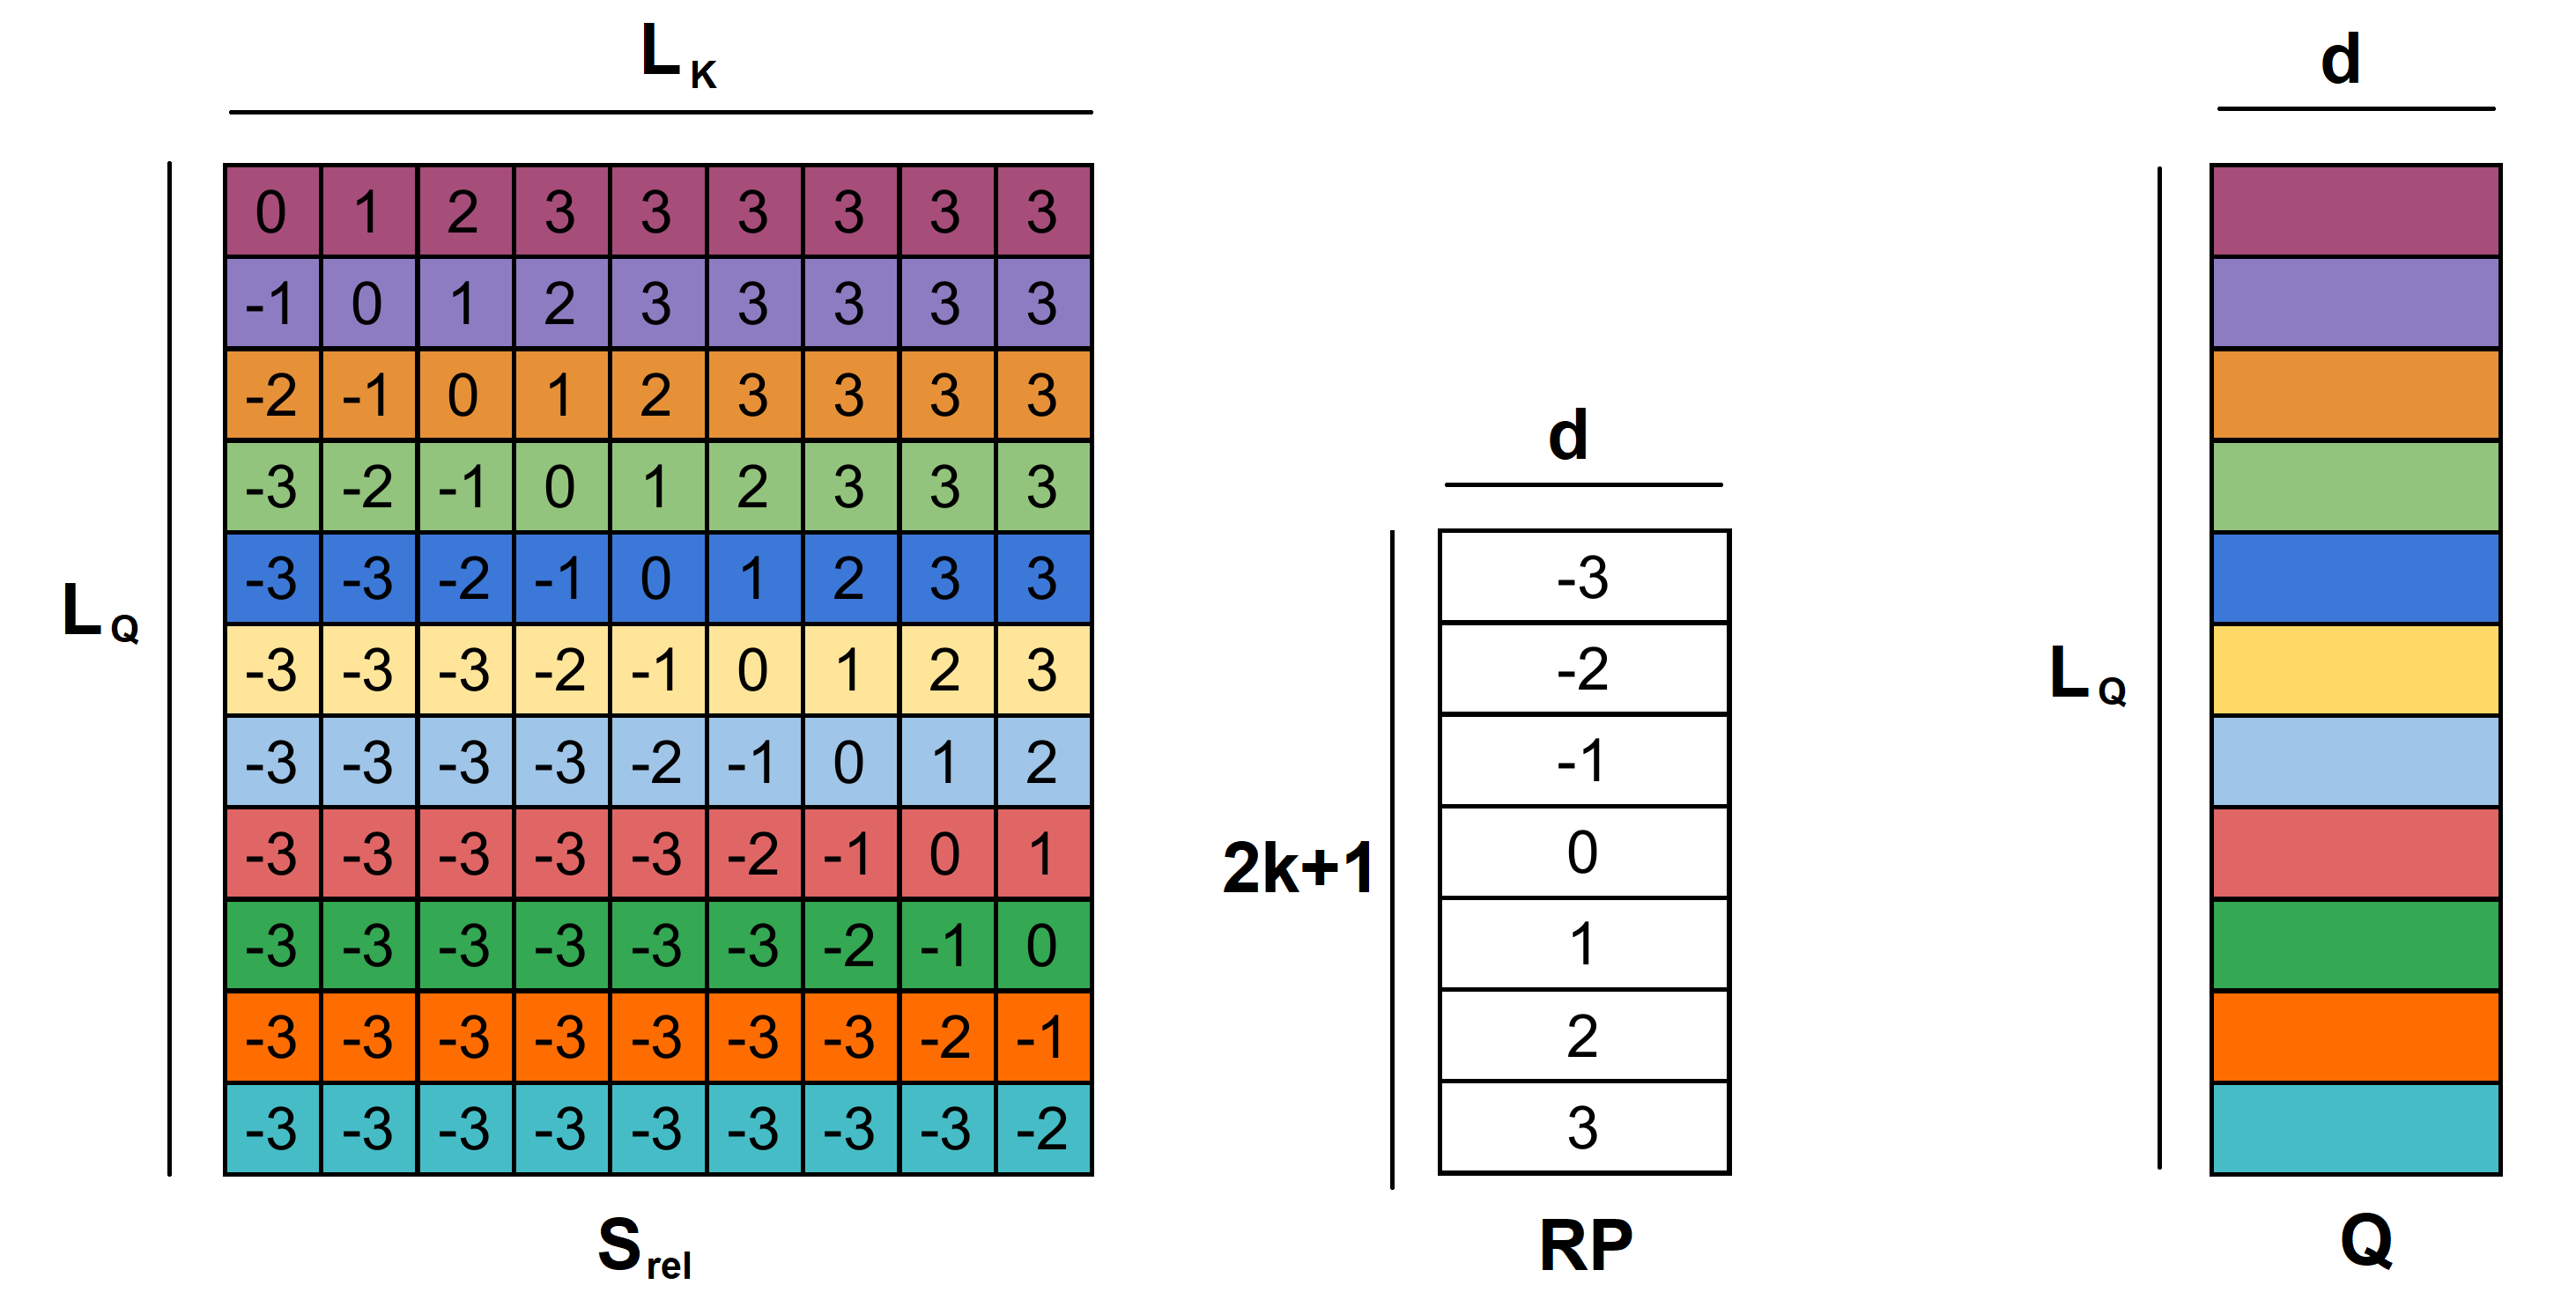
\includegraphics[width=0.9\linewidth]{images/S_rel.png}
\caption{$S_{rel}$ calculation}
\end{figure}

This score matrix must then be multiplied by the matrix of value
vectors: $A_{rel} = S_{rel} \times V$. Each row can be interpreted as
a set of weights in the weighted sum of the value vectors.

\begin{figure}
\centering
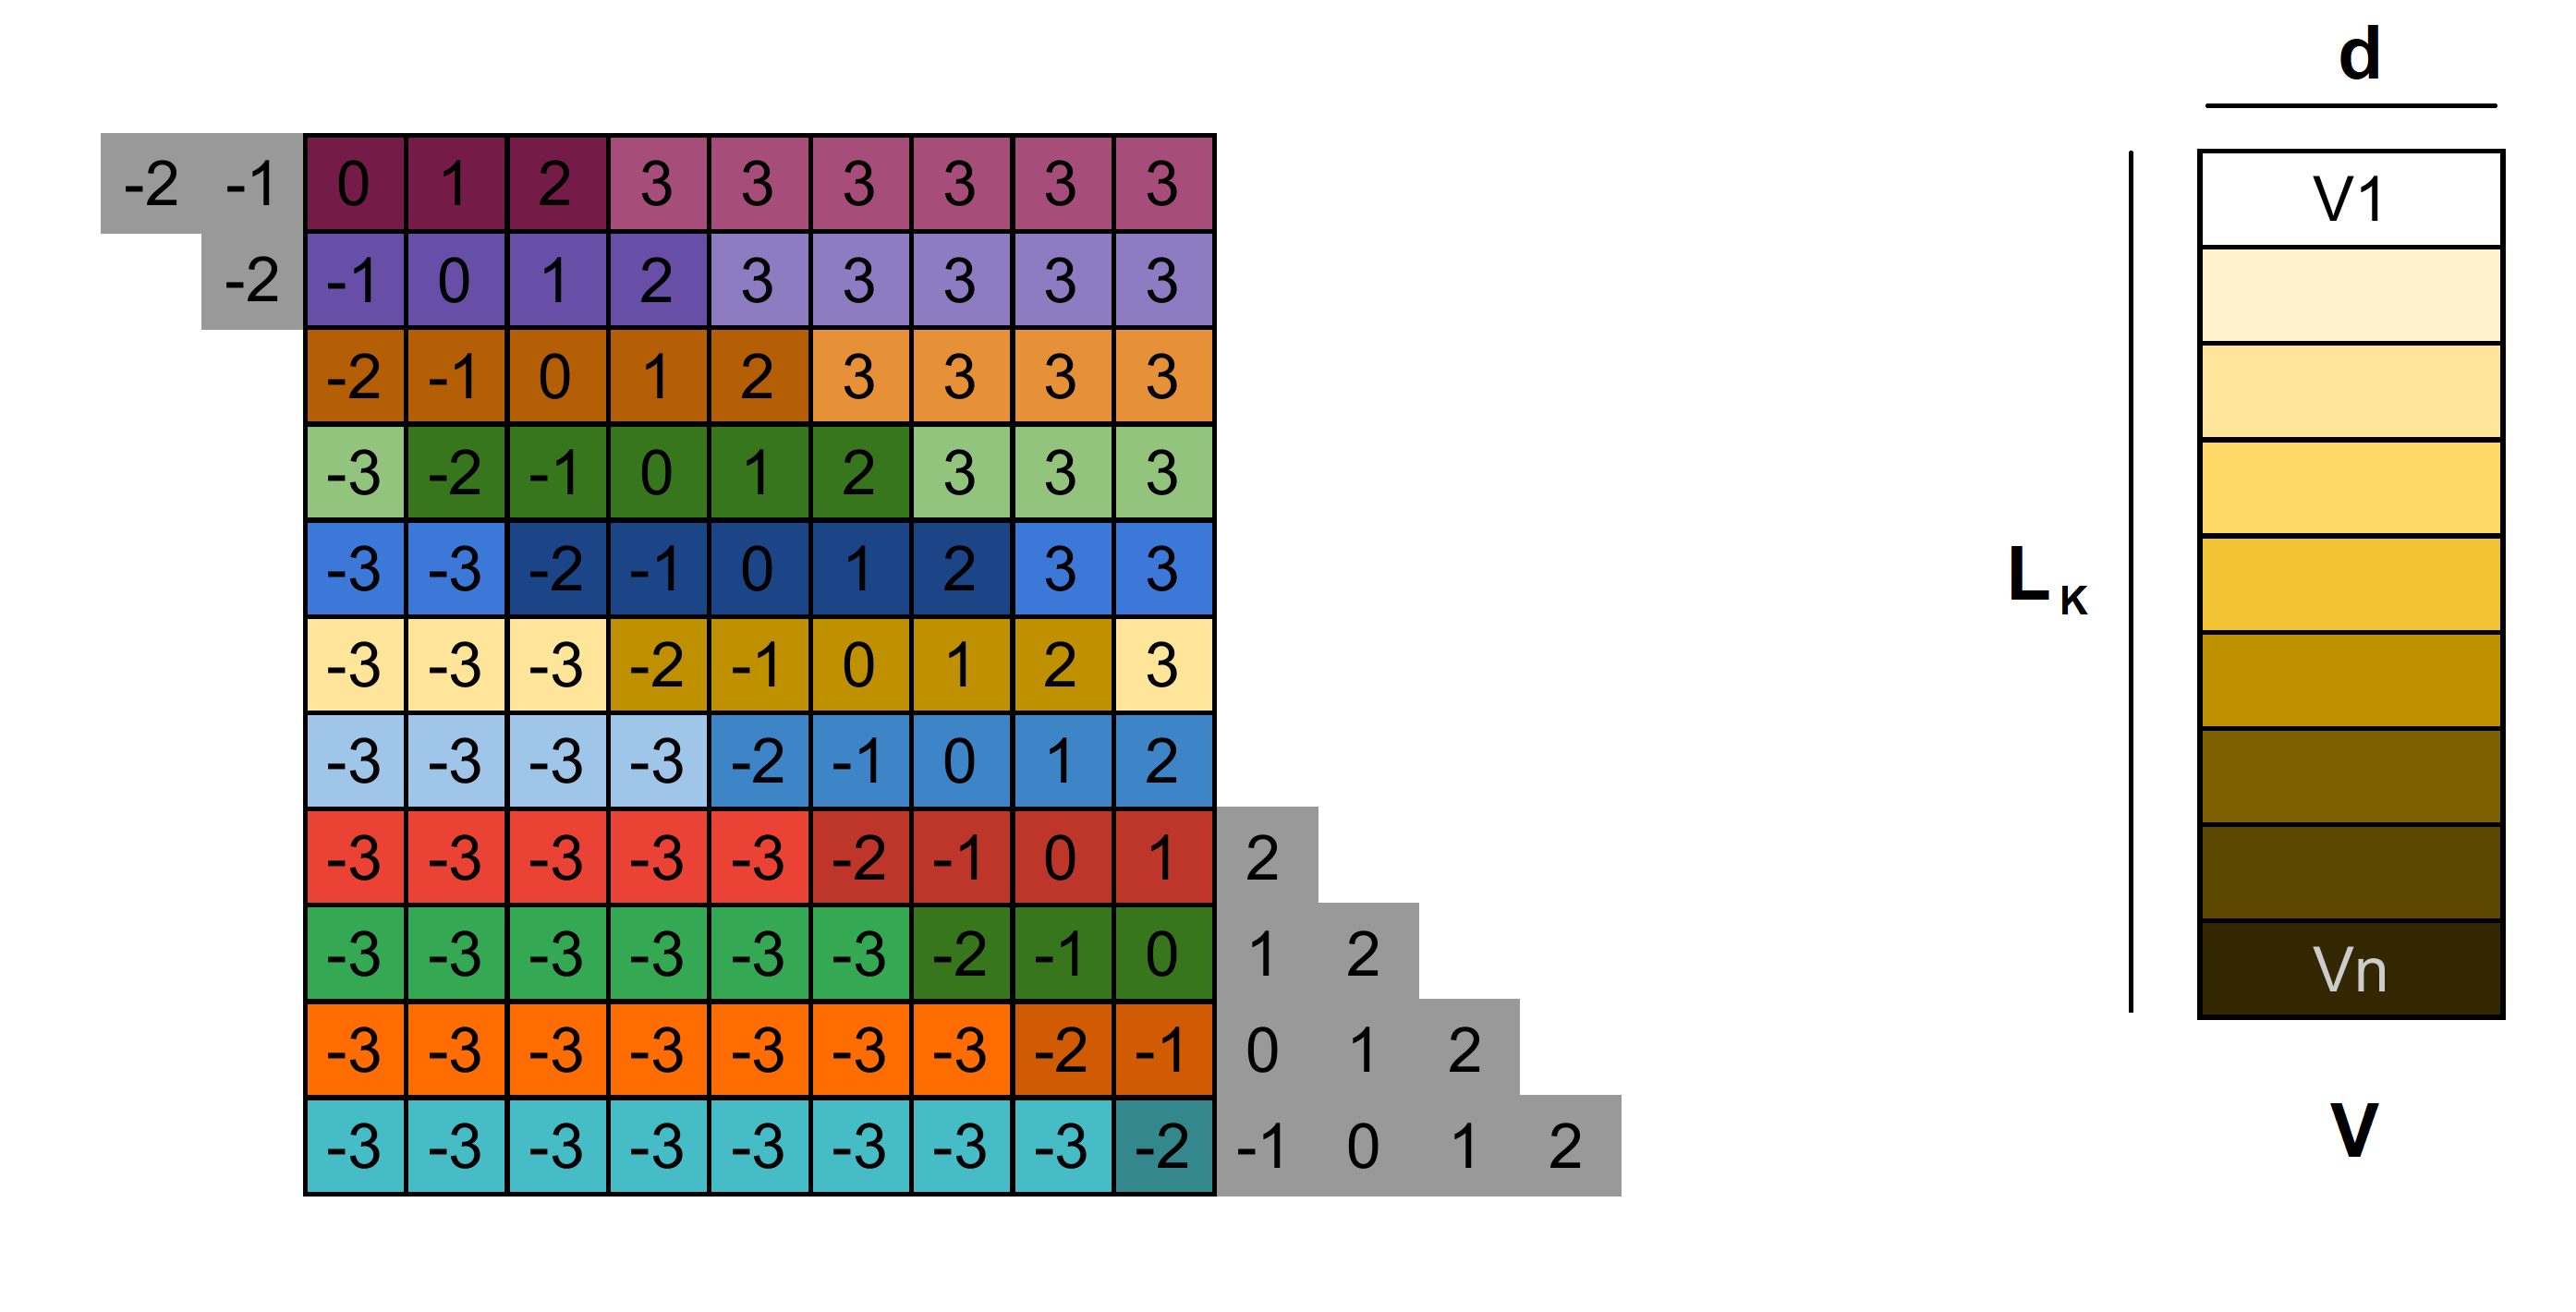
\includegraphics[width=0.9\linewidth]{images/S_rel_V.png}
\caption{$A_{rel}$ calculation}
\end{figure}

One can observe that the some weights are repeated several times in the
$S_{rel}$ matrix. So calculating the whole matrix can be avoided by
instead calculating the dot product of each query vector with each
relative position's embedding (complexity
$O \left(L_Q\times d\times(2k+1)\right)$). The operation can then be
decomposed in three terms: the lower triangle, the diagonal and the
upper triangle respectively.

\begin{itemize}
\item A set of weights that multiply a
accumulated sum of value vectors (complexity $O(max(L_Q, L_K))$)
\item An
element-wise multiplication between two tensors (complexity
$O(L_Q\times (2k-1) \times d)$)
\item A set of weights that multiply a
accumulated sum of value vectors (complexity $O(max(L_Q, L_K))$).
\end{itemize}

\begin{figure}
\centering
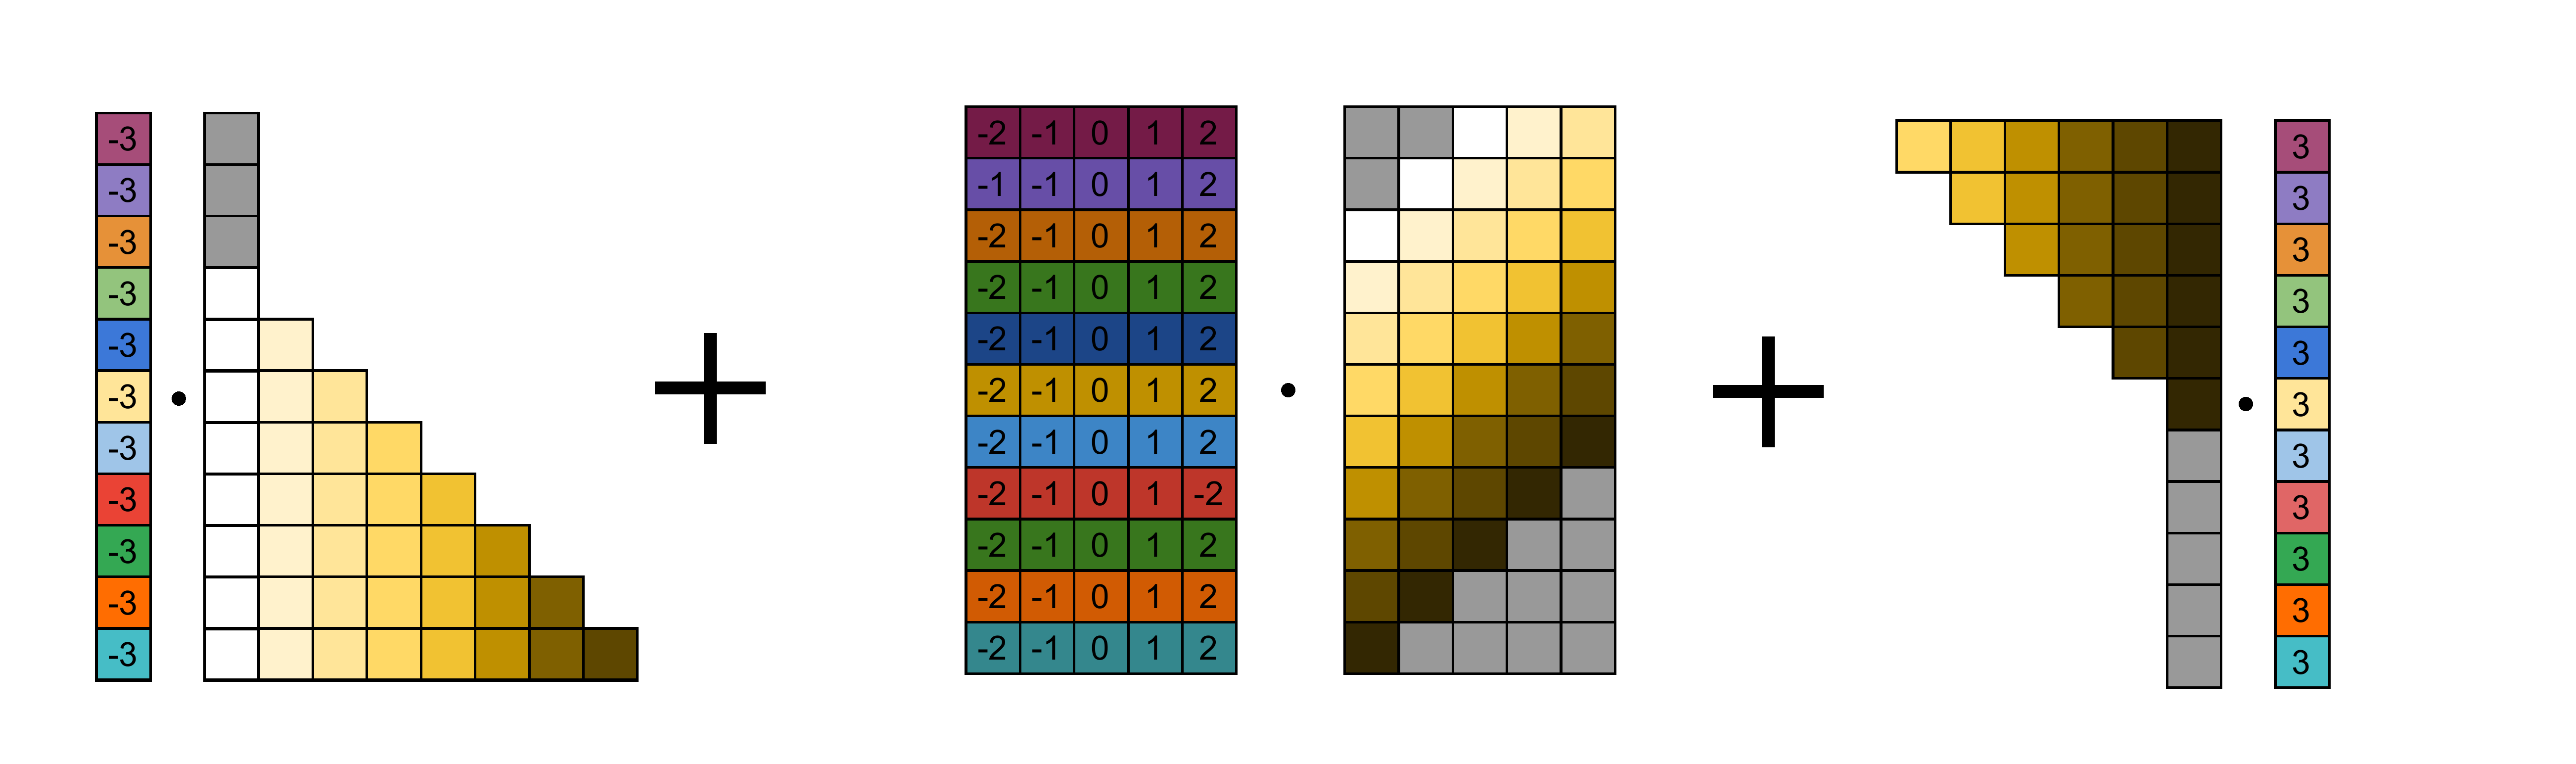
\includegraphics[width=0.9\linewidth]{images/S_rel_V_detailed.png}
\caption{$A_{rel}$ simplified calculation}
\end{figure}

Thus the attention can in fact be computed with linear complexity if we
get rid of the softmax function.

The memory used can be further reduced by observing that the right side
of the second element is a strided view of a padded copy of the value
matrix. Moving of one cell along the first dimension is equivalent to
moving along one cell of the second dimension.

The calculation can be implemented as follow, using zero-based slice
notation for compactness:

\begin{itemize}
	\item
	$\phi(Q)$, $\phi(V)$ and $RP$, are matrices of shape
	$(L_Q, d)$, $(L_K, d)$ and $(2k+1, d)$ respectively
	\item
	The dot product of each query and each relative position embedding is
	calculated as $weights = \phi(Q) \times RP^T$
	\item
	The weights of the horizon before and after are
	$H_{before} = weights_{[:, 0]}$ and
	$H_{after} = weights_{[:, -1]}$
	\item
	The weights of the diagonal are defined as
	$window = weights_{[:,1:-1]}$. For the masked case, columns on the
	right of the $k^{th}$ columns are set to 0
	($window_{[:, k+1:]} = 0$)
	\item
	The left term is calculated as
	$left = H_{before} * align(lower, min(max(0, L_Q-k), L_K))$ with
	$lower$ the concatenation of:
	
	\begin{itemize}
		\item
		a tensor of zeros of shape $\left(min(k, L_Q), d\right)$
		\item
		$cumsum(V, dim=0)$
	\end{itemize}
	\item
	The middle term is calculated as $middle = diagonal \odot strided$
	with $strided$ the strided view of:
	
	\begin{itemize}
		\item
		a tensor of 0 of shape $(max(0, k-1), d)$
		\item
		the value matrix $V$
		\item
		a tensor of shape $(max(0, L_Q-L_K), d)$
	\end{itemize}
	\item
	The right term is calculated as $right = 0$ for masked case, or for
	bidirectional case, $right = H_{right} * reverse$, with reverse the
	concatenation of:
	
	\begin{itemize}
		\item
		a tensor of 0 of shape $(L_Q-max(0, L_K-k), d)$
		\item
		$sum(V_{[inf, sup]}, dim=0) - cumsum(V_{[inf, sup-1]}, dim=0)$
		with $inf = k-1$, $sup = min(L_Q+k, L_K)$
	\end{itemize}
	\item
	The resulting attention function is $A = left + middle + right$
\end{itemize}

with:

\begin{itemize}
	\item
	$*$ the element-wise multiplication
	\item
	$\odot$ the element-wise multiplication followed by sum along second
	dimension
	\item
	all concatenations done along the first dimension
\end{itemize}

\endinput

\begin{algorithm*}[ht]
	\caption{calculation of $A^{rel}$ with linear complexity}
	\label{alg:A_rel}
	\KwIn{$\phi(Q)$ query vectors, tensor of shape $(L_Q, d)$}
	\NextInput{$\phi(RP)$ relative position embeddings, of shape $(2k+1, d)$}
	\NextInput{$V$ value vectors, tensor of shape $(L_K, d)$}
	\vskip12pt
	\KwData{$W$ tensor of shape $(L_Q, 2k+1)$}
	\NextData{$n_{before} := min(max(0, L_Q-k), L_K)$, scalar}
	\NextData{$p_{before} := min(k, L_Q)$, scalar}
	\NextData{$Cumulated$ tensor of shape $(L_Q, d)$}
	\NextData{$Summed$ tensor of shape $(d)$}
	\NextData{$Rcumulated$ tensor of shape $(L_Q, d)$}
	\NextData{$W^{horizon}$ tensor of shape $(L_Q, 2k-1)$}
	\NextData{$V^{horizon}$ tensor of shape $(L_Q, 2k-1, d)$}
	\NextData{$n_{after} := min(L_Q+k, L_K)$, scalar}
	\NextData{$p_{after} := max(0, Lq-max(0, Lk-k))$, scalar}
	\vskip12pt
	\KwResult{$A_{rel}$ tensor of shape $(L_Q, d)$}
	\vskip12pt
	$W := \phi(Q) \times \phi(RP)^T$\\
	\vskip3pt
	$Cumulated := cumsum(V, dim=0)$\\
	\vskip3pt
	$W^{before}_{i} := W_{i,0}$\\
	\vskip3pt
	$V^{before}_{ij} := 
	\begin{cases}
		0 & \text{if }i < p_{before}\\
		Cumulated_{i-p_{before}, j} & otherwise\\
	\end{cases}$\\
	\vskip3pt
	$A^{before}_{ij} := W^{before}_{i} \times V^{before}_{ij}$\\
	\vskip3pt
	$W^{horizon}_{ij} := W_{i+1,j}$\\
	\vskip3pt
	$V^{horizon}_{ijl} :=
	\begin{cases}
		V_{i-k+1+j, l} & \text{if }0 \leq (i-k+1+j) < L_K\\
		0 & \text{otherwise} 
	\end{cases}$\\
	\vskip3pt
	$A^{horizon}_{il} := \sum_j \left( W^{horizon}_{ij} \times V^{horizon}_{ijl} \right)$\\
	\vskip3pt
	$Summed_{j} := \sum_i \left( V_{ij}\right)$\\
	\vskip3pt
	$Rcumulated_{ij} := 
	\begin{cases}
		Summed_{j} & \text{if }i=0\\
		Summed_{j} - Cumulated_{i-1,j} & otherwise
	\end{cases}$\\
	\vskip3pt
	$W^{after}_{i} := W_{i, 2k}$\\
	\vskip3pt
	$V^{after}_{ij} := 
	\begin{cases}
		Rcumulated_{i+k-1,j} & \text{if }i<n_{after}\\
		0 & otherwise
	\end{cases}$\\
	\vskip3pt
	$A^{after}_{ij} := W^{after}_{i} \times V^{after}_{ij}$\\
	\vskip3pt
	$A^{rel}_{ij} := A^{before}_{ij} + A^{horizon}_{ij} + A^{after}_{ij}$
\end{algorithm*}

\endinput
\section{Linear Scalable Transformer
model}

As stated earlier, the proposed model proposes the replacement of the
scaled dot-product attention from original Transformer architecture by a
kernelized attention with relative positional encoding

The proposed model replaces the scaled-dot-product-attention by a
kernelized attention with RPE. Following the observations of
\citet{shaw2018selfattention} that
accumulating absolute positional encoding with relative positional
encoding yield no benefits, the positional encoding is also removed -
although for some specific applications it might be beneficial to
maintain it. The algorithm used to calculate each term is chosen
dynamically to occupy the least memory depending on the sequence lengths
and embedding dimensions - as memory usage is easier to evaluate
precisely than execution time.

In this work we have chosen the following formulation, with
$\phi(x) = elu(x) + 1$.

\begin{equation}
A = \frac{\left( \phi(Q) \times \phi(K^T) + S^{rel} \right)}{\sum_j \left( \phi(Q) \times \phi(K^T) + S^{rel} \right)} \times V
\end{equation}

This is essentially a combination of two terms: the kernelized attention
proposed by  \citet{katharopoulos2020transformers}, and the relative positional encoding proposed by
\citet{shaw2018selfattention}. The left
term is the score matrix of shape $(L_Q, L_K)$, with a denominator
which scales all rows so that they sum to 1. For the sake of the
implementation, the multiplication must be distributed as:

\begin{equation}
A = \frac{\left( \phi(Q) \times \phi(K^T) \times V \right) + \left( S^{rel} \times V\right)}{\sum_j \left( \phi(Q) \times \phi(K^T) \right) + \sum_j \left( S^{rel} \right)}
\end{equation}

The denominator can be easily calculated by applying the (naive or
linear complexity) algorithms with V replaced by a matrix of shape
$(L_K, 1)$ full of 1.

For each case (masked/bidirectional) the algorithm is chosen between
naive and linear complexity to occupy the least memory.

\begin{itemize}
\item
for the masked $Q \times K^T \times V$ term, the memory occupied by
the naive algorithm is $L_QL_K$ while the linear complexity
algorithm occupies $d^2 \times max(L_Q, L_K)$
\item
for the bidirectional $Q \times K^T \times V$ term, the memory
occupied by the naive algorithm is $L_QL_K$ while the linear
complexity algorithm occupies $d^2$
\item
for the $S_{rel} \times V$ term (masked and bidirectional), the
memory occupied by the naive algorithm is $L_QL_K$ while the linear
complexity algorithm occupies $L_Q \times (2k+1 + 4)$
\end{itemize}

\endinput

\begin{figure*}
	\begin{minipage}{0.48\textwidth}
		\centering
		\captionsetup{justification=centering}
		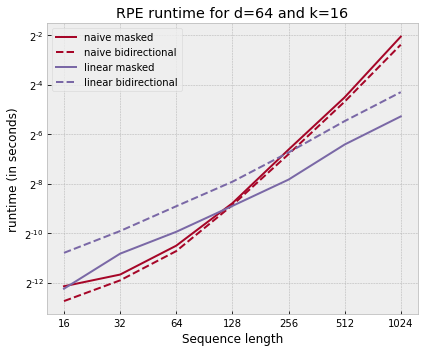
\includegraphics[width=1\linewidth]{images/runtimes_RPE.png}
		\caption{$S^{rel} \times V$ calculation runtimes for $d=64$ and $k=16$}
		\label{fig:RPE_timings}
	\end{minipage}\hfill
	\begin{minipage}{0.48\textwidth}
		\centering
		\captionsetup{justification=centering}
		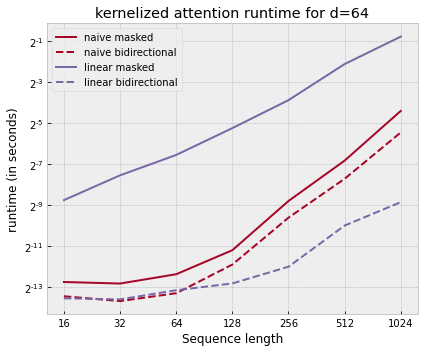
\includegraphics[width=1\linewidth]{images/runtimes_KA.png}
		\caption{$\phi(Q) \times \phi(K^T) \times V$ calculation runtimes for $d=64$}
		\label{fig:kernelized_attention_timings}
	\end{minipage}
\end{figure*}
\section{Results}

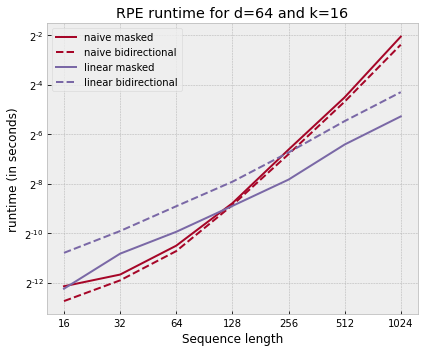
\includegraphics[width=0.9\linewidth]{images/runtimes_RPE.png}

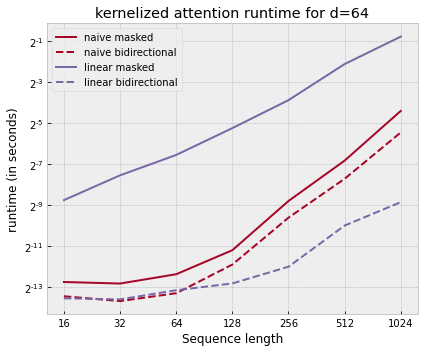
\includegraphics[width=0.9\linewidth]{images/runtimes_KA.png}

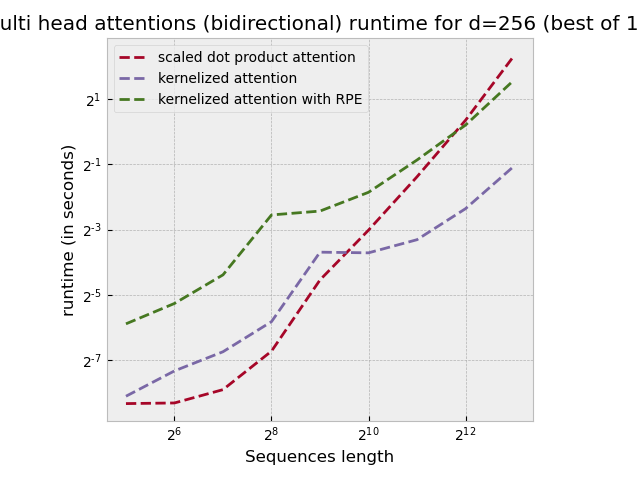
\includegraphics[width=0.9\linewidth]{images/runtimes_MHA.png}

\endinput

\section{Conclusion}

In the present work an easily implemented algorithm to compute
\citet{shaw2018selfattention} relative
positional embedding with linear complexity has been presented. An
implementation of \citet{choromanski2021rethinking} prefix sum algorithm that doesn't requires custom CUDA
code (while maintaining linear complexity) was also presented.

These two elements allowed to define a kernelized attention function
with relative positional encoding, that can be computed with linear
complexity with regards to sequence length. The proposed model presents
linear scalability with sequence length, can be implemented out-of-the-box in neural network framework, and is adapted to sequence to sequence
problems instead of being restricted to encoders only models.

\endinput

\section*{Table of symbols}

\begin{tabular}{cp{0.5\textwidth}}
	$\boldsymbol{A}$ & the result of the attention operation, tensor of shape ($L_Q$, $d$)\\
	$\boldsymbol{d}$ & the projection dimension\\
	$\boldsymbol{D}$ & the embedding dimension\\
	$\boldsymbol{h}$ & the number of heads\\
	$\boldsymbol{k}$ & the radius of the attention horizon\\
	$\boldsymbol{K}$ & the keys linked to the attended sequence, tensor of shape ($L_K$, $d$)\\
	$\boldsymbol{L_K}$ & the sequence length of the attended sequence\\
	$\boldsymbol{L_Q}$ & the sequence length of the transformed sequence\\
	$\boldsymbol{Q}$ & the query linked to the sequence to transform, tensor of shape ($L_Q$, $d$)\\
	$\boldsymbol{RP}$ & The relative position embeddings, tensor of shape ($2k+1$, $d$)\\
	$\boldsymbol{S_{rel}}$ & The matrix of relative position scores, tensor of shape ($L_Q$, $L_K$)\\
	$\boldsymbol{V}$ & the values linked to the attended sequence, tensor of shape ($L_K$, $d$)\\
\end{tabular}

\endinput

\end{multicols}{}
\clearpage

\bibliography{paper-scaleformer}

\end{document}
